\chapter{Graph Cubes: State of the Art}
% ---

This chapter presents the most important research works published in the area of OLAP systems implemented using graph databases. The first work presented here dates back to 2011 and introduces several concepts - such as graph cube, aggregate graphs and cuboid queries - that serve as basis for other papers published since then.

\section{Graph Cube: On Warehousing and OLAP Multidimensional Networks}

One of the main works in graph analysis using OLAP methods is described in \cite{Zhao2011}, and it  introduces several concepts that will be used by other authors to describe their work in this area. Graph Cube is one of those concepts and it is defined as a multidimensional model that extends multidimensional networks to provide decision support features. A multidimensional network is a graph $N=(V,E,A)$, where $V$ is a set of vertices, $E$ is a set of edges and $A$ is a set of vertex-specific attributes. Each vertex in the graph is a multidimensional tuple and the attributes of the vertex define the graph cube dimensions.
 
A graph cube is formed by all possible aggregate networks calculated from the original multidimensional network. An aggregate network (often called cuboid) is a summarisation of the original graph with respect to one or more dimensions, which is calculated by applying an aggregate function (e.g. COUNT, SUM, AVERAGE, among others) on the vertices attributes. Consider the multidimensional network illustrated in Figure \ref{fig:figure12}.

\begin{figure}[ht]
\centering
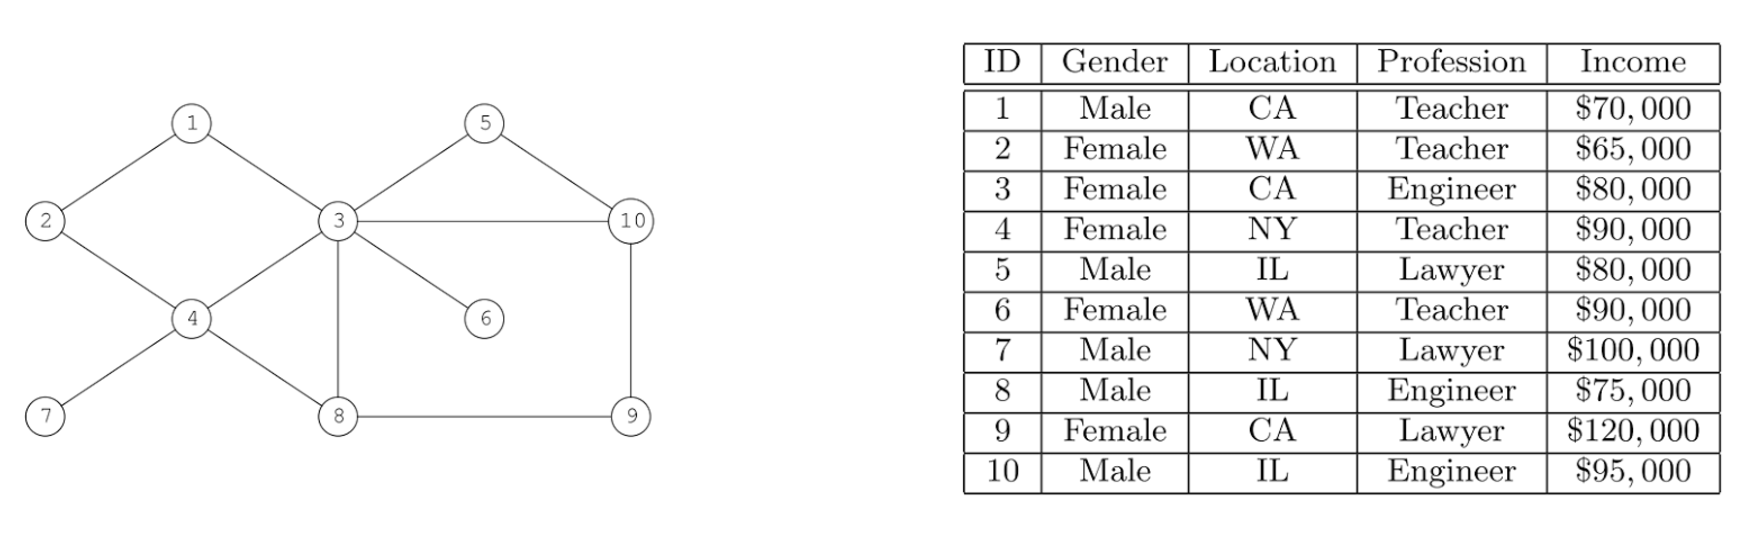
\includegraphics[width=1\textwidth]{../multidimensional_graph.png}
\caption{Multidimensional network \cite{Zhao2011}}
\label{fig:figure12}
\end{figure}

\begin{figure}[ht]
\centering
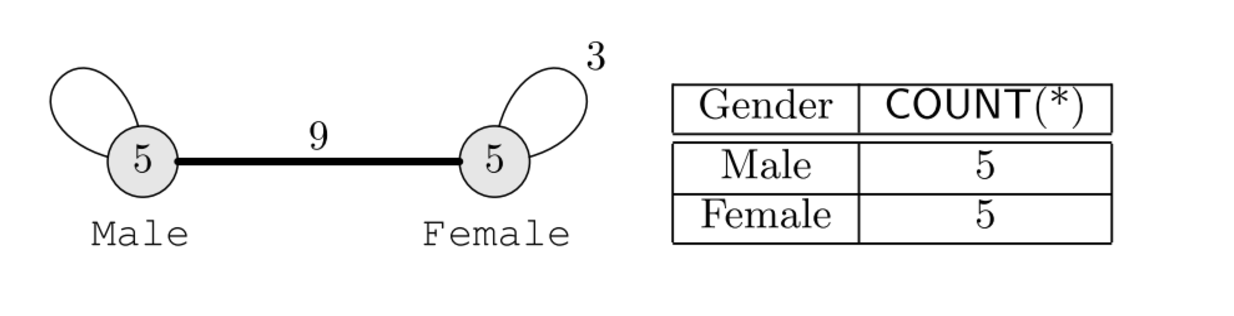
\includegraphics[width=0.8\textwidth]{../aggregate_graph.png}
\caption{Aggregate Network by \emph{Gender} dimension \cite{Zhao2011}}
\label{fig:figure13}
\end{figure}

The vertices of the graph presented in Figure \ref{fig:figure12} represent individuals and the edges represent the relationship between these individuals. The table on the right side of Figure \ref{fig:figure12} describes the attributes of each vertex: an unique \emph{ID}, \emph{Gender}, \emph{Location}, \emph{Profession} and \emph{Income}. Figure \ref{fig:figure13} shows the cuboid obtained by applying the function COUNT on the attribute \emph{Gender}: two vertices represent the possible values for the attribute (Male and Female) and they contain the number of vertices in the original graph with the respective \emph{Gender} value. It is important to notice that the relationship between individuals was also aggregated in the resulting network, e.g. the aggregate network show that there are 9 relationships between male and female individuals in the original graph, which is represented by an edge with weight of 9.

The dimension of a cuboid is given by the set of non-aggregate dimensions of the cuboid. For instance, the cuboid in Figure \ref{fig:figure13} has the dimension $\{Gender\}$. A cuboid $A'$ is an ancestor of another cuboid $A"$ if $dim(A')$ contains $dim(A'')$. Given these definitions, all possible cuboids of a graph cube can be organised in a graph cube lattice, ordering the cuboids according to its ancestors. A multidimensional network $N$ with $n$ dimensions has $2^n$ cuboids in the graph cube. Figure \ref{fig:figure14} shows the graph cube lattice for the multidimensional network introduced in Figure \ref{fig:figure12}, considering only \emph{Gender}, \emph{Location} and \emph{Profession} as dimensions.

\begin{figure}[ht]
\centering
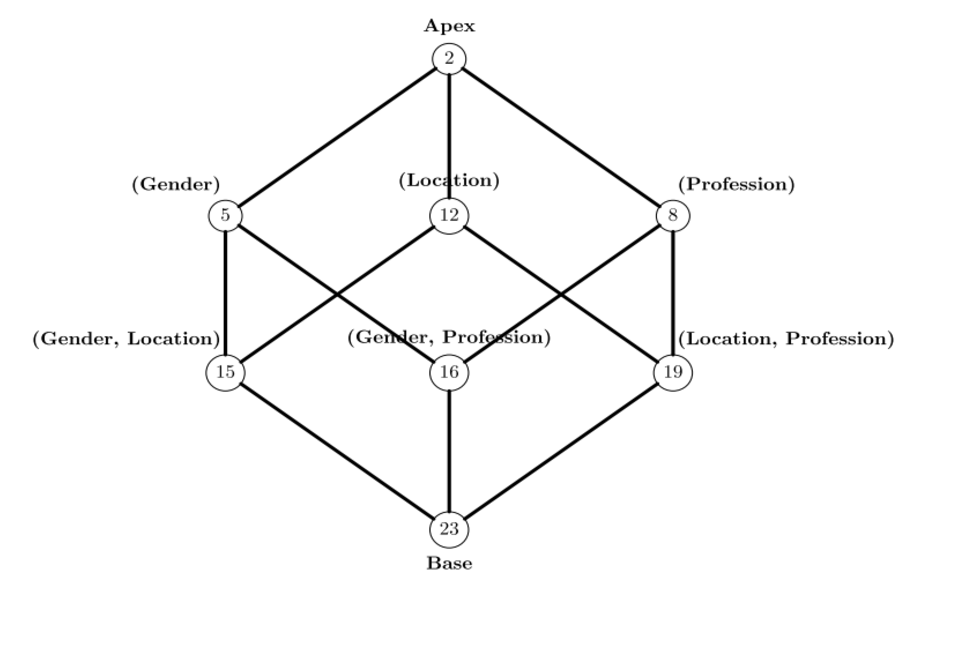
\includegraphics[width=0.6\textwidth]{../graph_lattice.png}
\caption{Graph Cube Lattice \cite{Zhao2011}}
\label{fig:figure14}
\end{figure}

The paper proposes two OLAP query models:
\begin{description}
\item[Cuboid Query] Aggregate vertices and edges based on the dimension requested in the query and can work with any aggregate function (SUM, AVG, etc). For instance, consider a graph with vertices containing the attributes (\emph{Gender}, \emph{Location}, \emph{Profession}). A cuboid query for this graph can be $(Gender, *, *)$ which will result in an aggregate graph showing all the vertices with the same Gender value aggregated and the edges also aggregate by the function COUNT.
\item[Crossboid Query] Return the aggregate network between two or more cuboids structures. An example of a crossboid query can be the aggregate network between an user with $ID = 3$ and all the locations.
\end{description}

Given that the size of the graph cube lattice is exponential with respect to the number of dimensions of the original multidimensional network, the paper proposes a partial materialisation in order to process queries. The partial materialisation is implemented using a greedy algorithm that selects k cuboids $(k < 2^n)$ to be materialised according to the benefit of those cuboids to improve the cost for query evaluation.
 
The graph cube implementation described above is also studied by other works. In \cite{Denis2013}, a distributive approach is proposed using map reduce jobs to calculate each step of the aggregation process. In \cite{Khan2014}, a new algorithm to compute the Graph Cube (iGraphCubing) is proposed, using a new prunning method based on the Structural Significance measure.This measure takes into account three factors:
 
\begin{itemize}
\item The diversity of the attribute value in the neighborhood for each vertex
\item The clustering coefficient
\item The density around each vertex
\end{itemize}

The work in \cite{Zhao2011} presents experiments evaluating the effectiveness and the efficiency of the method proposed. The effectiveness was evaluated by analysing OLAP queries submitted to the graph cube. The efficiency was evaluated by analysing the graph cube performance depending if it was fully or partially materialised in disk. In conclusion, the paper proposes an implementation of a graph cube obtained from an homogeneous attributed graph, but it does not consider heterogeneous networks neither attributed edges.

\section{Graph OLAP: Towards Online Analytical Processing on Graphs}

The Graph OLAP framework  proposed in \cite{Chen2008} takes as input a set of network snapshots, where each snapshot contains a graph and a set of informational attributes that describes the snapshot. In this scenario, the paper defines two dimension types: informational dimensions (formed by the informational attributes) and topological dimensions (formed by the attributes of the vertices and edges of the graph). The authors distinguish different semantics for OLAP operations in graphs, so these operations are categorised into Informational OLAP (I-OLAP) and Topological OLAP (T-OLAP).

The framework gives as output an aggregate graph with a summarised view of the snapshots set. The type of the aggregate graph returned by the framework can also be categorised in Informational Aggregate Graph (I-aggregate graph) and Topological Aggregate Graph (T-aggregate graph). 
 
Informational Aggregate Graph is computed based on a set of network snapshots that have informational dimensions with same values. Figure \ref{fig:figure15} shows an example of an i-aggregate graph composed by snapshots describing the co-author relationship between individual authors. The co-author relationship is grouped by a certain conference (\emph{sigmod}, \emph{vldb}, \emph{icde}), by a class of conferences (\emph{db-conf}), by a specific period of time (\emph{2004}, \emph{2005}) and by a group of time periods (\emph{all-years}). It is important to notice that the graph in Figure \ref{fig:figure15} shows different levels of aggregations for each co-author relationship. 

\begin{figure}[ht]
\centering
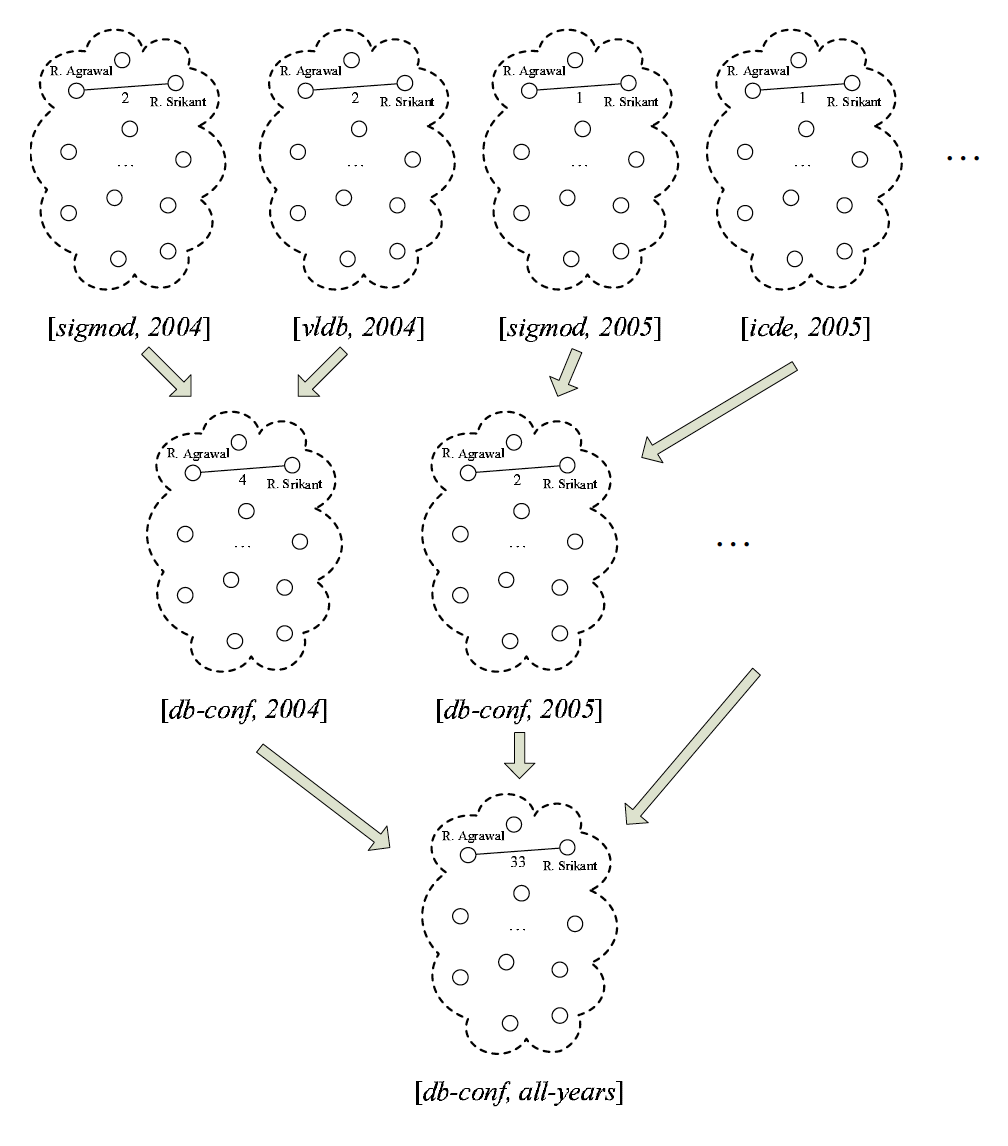
\includegraphics[width=0.6\textwidth]{../i_aggregated_graph_example.png}
\caption{Example of Informational Aggregate Graph \cite{Chen2008}}
\label{fig:figure15}
\end{figure}

Classic OLAP operations in an i-aggregate graph can be interpreted as follows:
\begin{description}
\item[Roll-up] Aggregate multiple snapshots to form a higher level summary of information
\item[Drill-down] Return to lower-level snapshots from aggregate graph
\item[Slice / dice] Select a subset of snapshots based on informational dimensions
\end{description}
 
Topological Aggregate Graph is obtained based on a single network, where the vertices are the result of applying the aggregate function to the vertices of the original network with the same attribute value. Figure \ref{fig:figure16} shows an example of a t-aggregate graph where the information about co-author relationship between individual authors in one snapshot was aggregated into co-author relationship between the institutions the authors belong to.

\begin{figure}[ht]
\centering
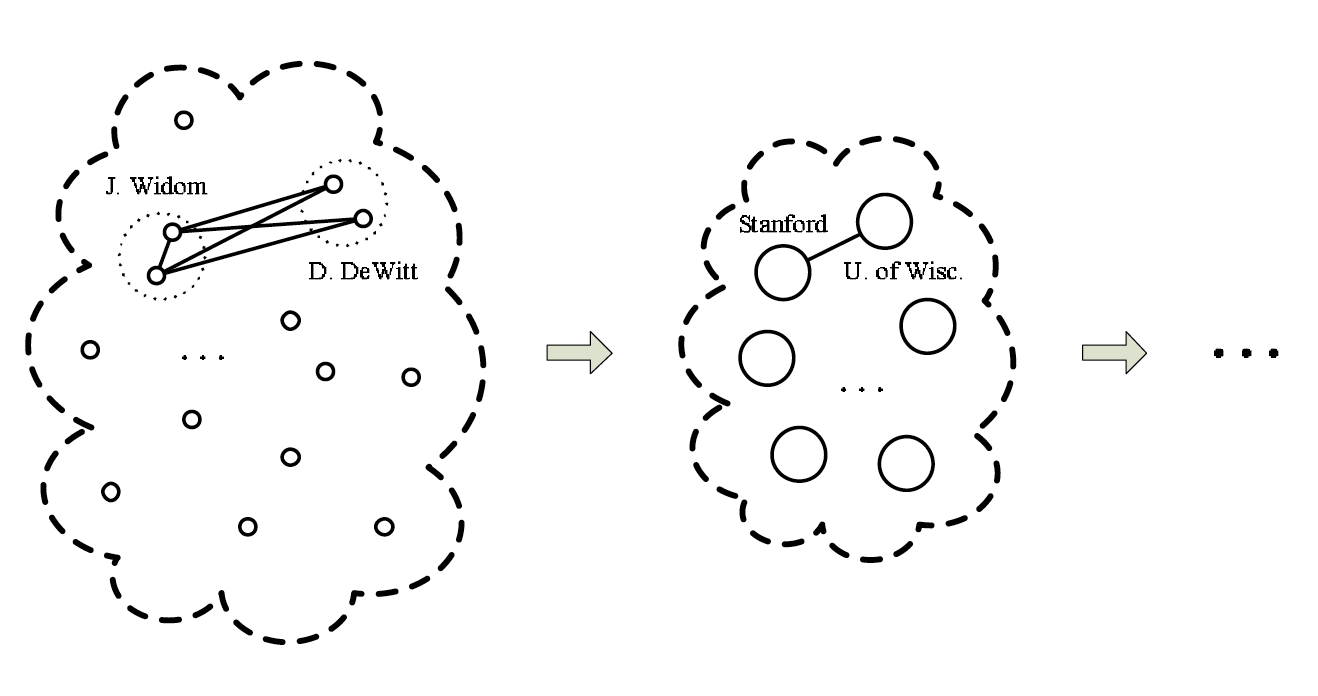
\includegraphics[width=0.7\textwidth]{../t_aggregated_graph_example.png}
\caption{Example of Topological Aggregate Graph \cite{Chen2008}}
\label{fig:figure16}
\end{figure}

Classic OLAP operations in an t-aggregate graph can be interpreted as follows:
\begin{description}
\item[Roll-up] Merge topological elements (vertices or edges) and replace them by corresponding higher-level elements
\item[Drill-down] Split merged elements into lower-level elements
\item[Slice / dice] Select a subgraph of a snapshot based on topological dimensions
\end{description}

The Topological OLAP is further explained in \cite{Qu2011}. This work takes into consideration two properties (T-Distributiveness and T-Monotonicity) used to classify how different measures can be performed in an OLAP Graph. A measure function is considered T-Distributive if the result of the function applied to high-level vertices from the graph can be obtained by the computation of pre-computed results of the same function applied to lower-level vertices from the same graph. On the other hand, a measure is considered T-Monotone, if the data search space can be pruned given a user-defined threshold, by dropping vertices pairs with measures that do not satisfy the threshold. The paper shows experiments using common constraint function, proven to be T-Distributives and/or T-Monotones, such as SUM, MIN, MAX, Density, Degree Centrality, Closeness Centrality, among others.

\section{HMGraph}

An Heterogeneous and Multidimensional Graph OLAP framework (HMGraph OLAP) is proposed in \cite{Yin2012}. This framework uses a graph model similar to Graph OLAP \cite{Chen2008}, but it adds the concept of Entity Dimensions due to the heterogeneity of the input graphs (Graph OLAP framework only handles homogeneous graphs). Figure \ref{fig:figure17} shows an example of a heterogeneous multidimensional network, highlighting the entity attributes of the graph.

\begin{figure}[ht]
\centering
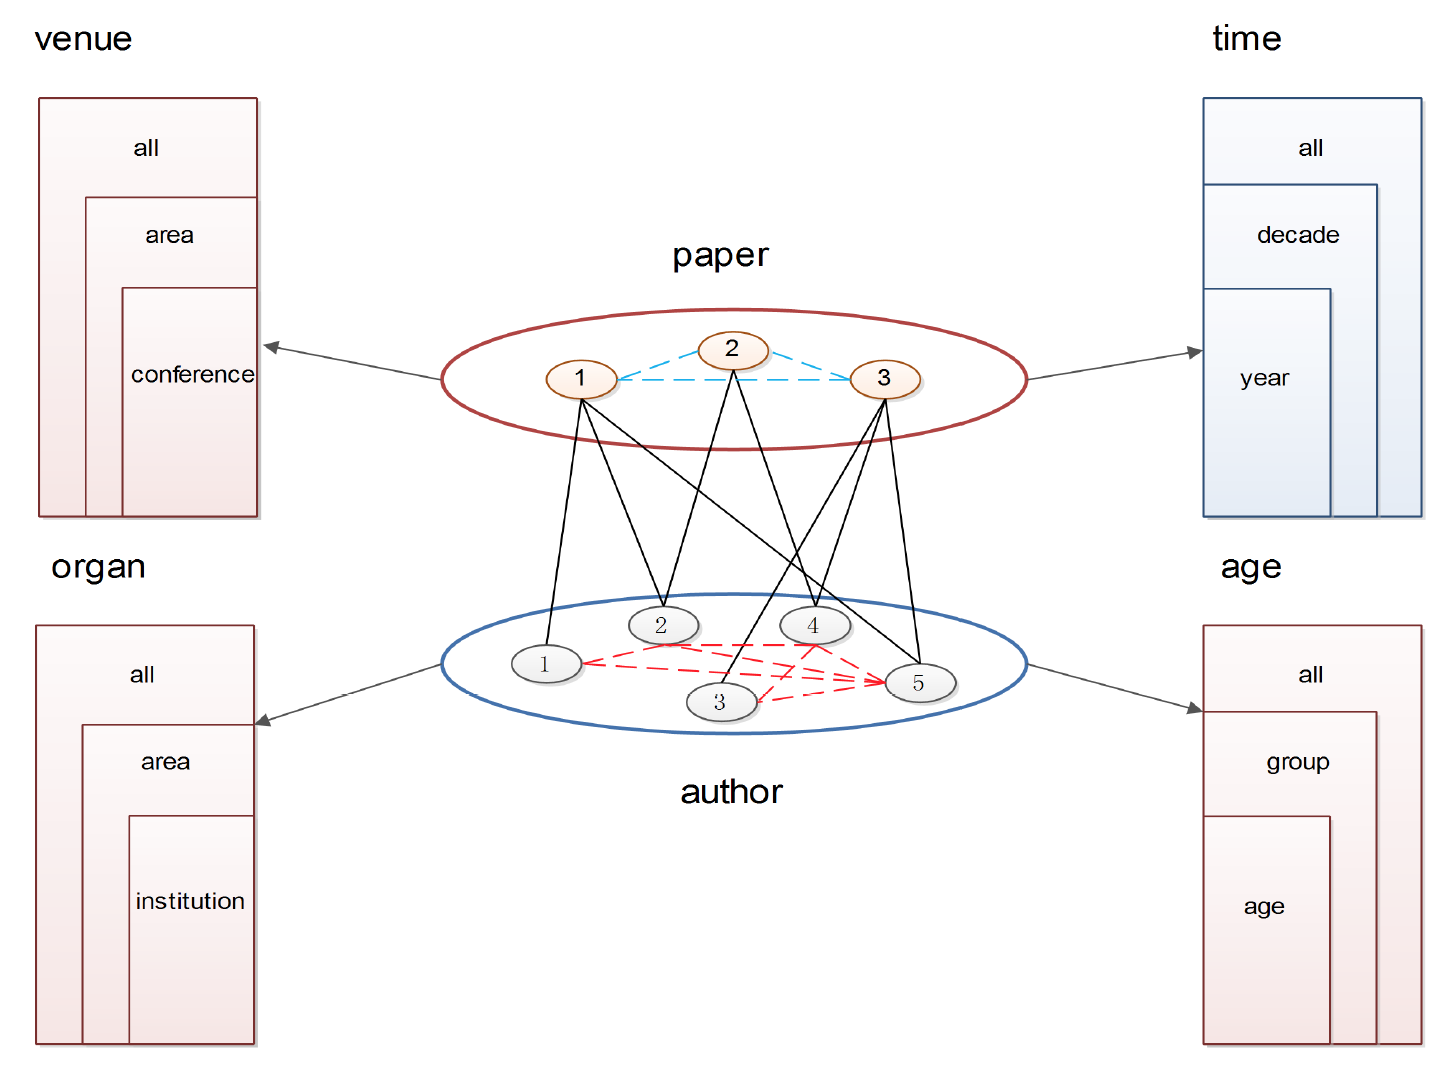
\includegraphics[width=0.7\textwidth]{../heterogeneous_graph_example.png}
\caption{Example of a heterogeneous multidimensional network \cite{Yin2012}}
\label{fig:figure17}
\end{figure}

Entity attributes are the attributes that describe the characteristics of an entity. In the graph illustrated in Figure \ref{fig:figure17}, organ and age are entity attributes of author entity. Entity Dimension is related to the types of vertices in the graph.

Like Graph OLAP, HMGraph can perform I-OLAP and T-OLAP operations, but it can also perform rotate and stretch operations. The rotate operation is done by changing vertices into edges and edges into vertices, as shown in Figure  \ref{fig:figure18}. The stretch operation is done by changing edges into entities and adding edges between the recently created entity and the vertices previously connected to the transformed edge, as shown in Figure \ref{fig:figure19}.

\begin{figure}[ht]
\centering
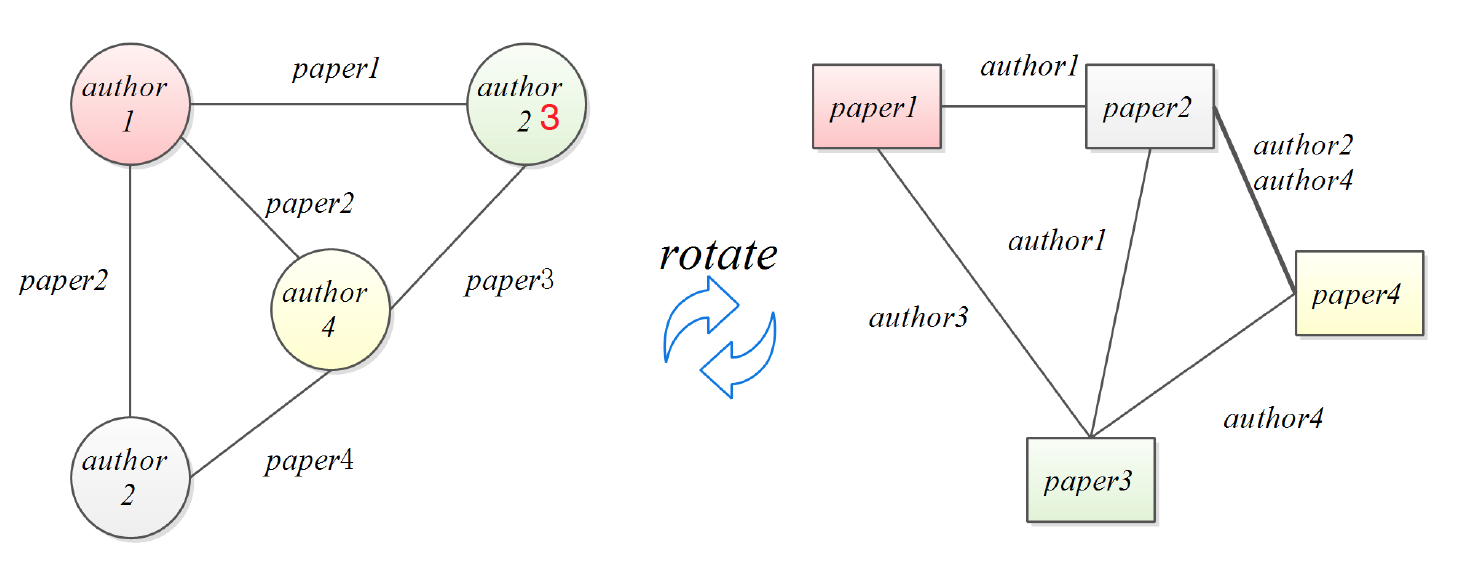
\includegraphics[width=0.7\textwidth]{../rotate_operation_example.png}
\caption{Example of rotate operation \cite{Yin2012}}
\label{fig:figure18}
\end{figure}

\begin{figure}[ht]
\centering
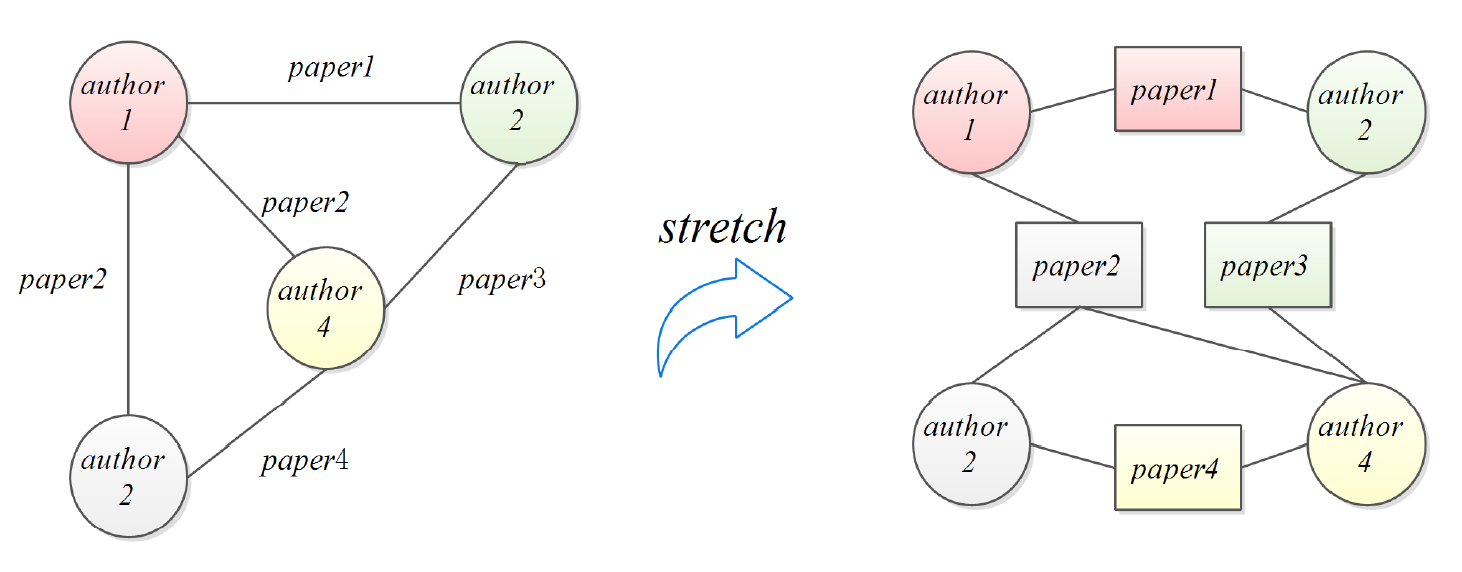
\includegraphics[width=0.7\textwidth]{../stretch_operation_example.png}
\caption{Example of stretch operation \cite{Yin2012}}
\label{fig:figure19}
\end{figure}

Even though the work presented in \cite{Yin2012} draws attention to the importance of heterogeneous networks in real world application, the paper does not provide further implementation detail on how the framework can be used with real data.

\section{Pagrol: PArallel GRaph OLap over Large-scale Attributed Graphs}

The work presented in \cite{Wang2014} proposes a parallel Graph OLAP system, adopting the Hyper Graph Cube model that extends attributed graphs to support decision making services. The model proposed in this paper is similar to the Graph Cube described in \cite{Zhao2011}, with the main difference being the presence of attributes also in the graph edges. In this scenario, there are two types of dimensions: vertex dimensions and edge dimensions. Figure \ref{fig:figure20} shows an example of an attributed graph.

\begin{figure}[ht]
\centering
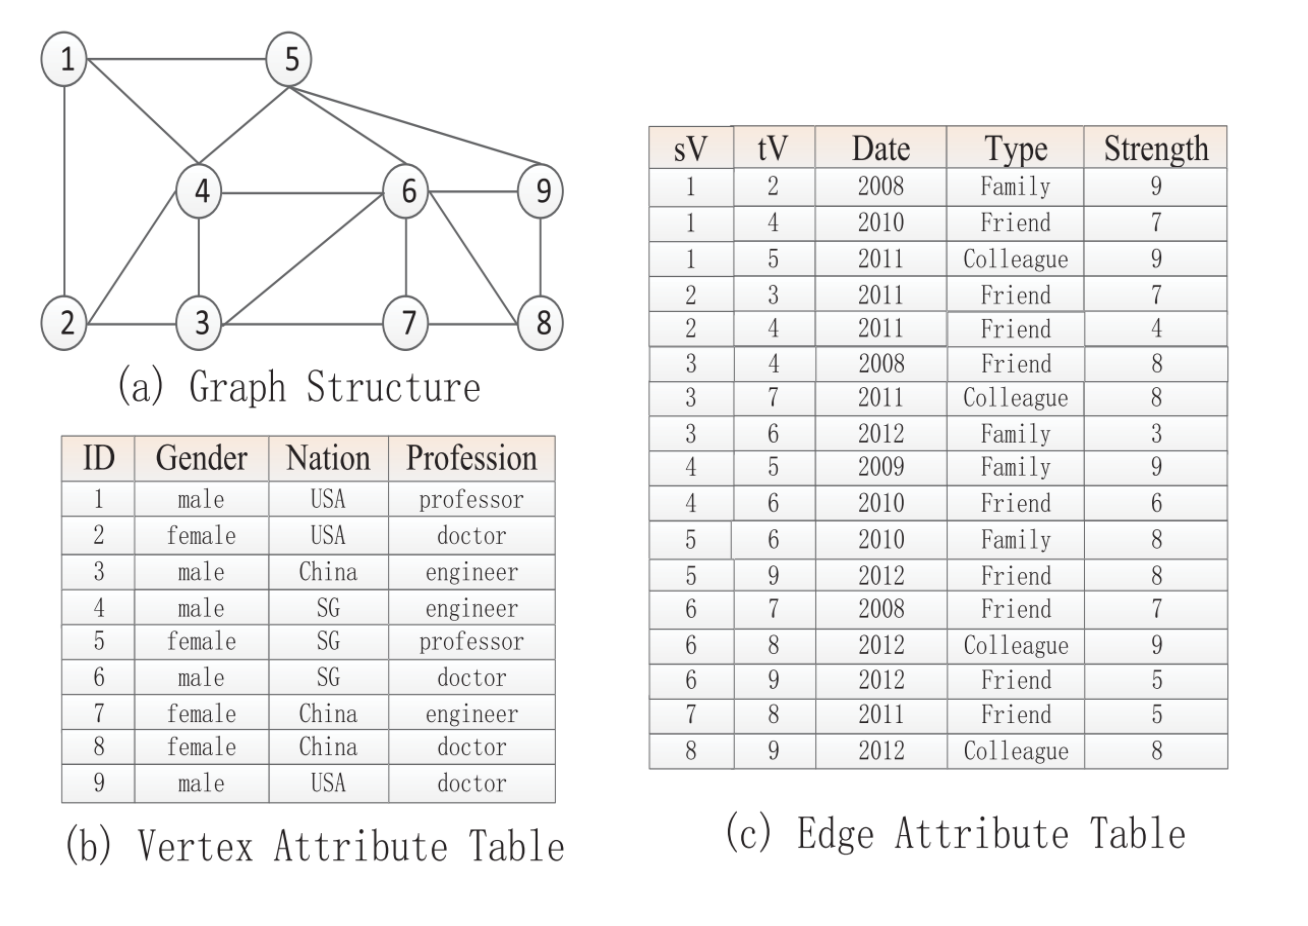
\includegraphics[width=0.8\textwidth]{../attributed_graph.png}
\caption{Example of attributed graph \cite{Wang2014}}
\label{fig:figure20}
\end{figure}

Given an attributed graph with n vertex dimensions and m edge dimensions, the Hyper Graph Cube will contain $2^{n+m}$ aggregate graphs obtained as described by the work of \cite{Zhao2011}. This Hyper Graph Cube can be seen as the cartesian product between all the vertex-aggregate networks (when one or more vertex dimensions are aggregated) and the edge-aggregate networks (when one or more edge dimensions are aggregated). This cube arrangement can support the following categories of queries:

\begin{description}
\item[Category 1] Queries answered by information stored either in a vertex or in an edge attributes. For example:``How many relationships appeared in 2012?'' or ``What is the percentage of users in each different profession in this network?''
\item[Category 2] Queries answered by integrating the knowledge stored at both vertex and edges attributes. For example: ``What is the trend of the number of relations appearing between USA and SG (Singapore) in the last 3 years?''
\item[Category 3] Queries answered by an aggregate graph, that provides a summarised view of the data along some dimensions. For example: ``What is the graph structure as grouped by users' gender as well as relationship type?''
\end{description}

The Hyper Graph Cube also supports roll-up and drill-down operations, along both vertex and edge dimensions. For instance, if we have an aggregate graph along Location dimension according to City value, we can roll up to obtain an aggregate graph according to State value.
 
The materialisation for the Hyper Graph Cube is done using Map-Reduce(MR) jobs. Since vertex and edges are stored in two different tables in the distributed file system (DFS), the materialisation is done in two steps: first the two tables are joined into one flat table containing all the dimensions and the second step performs the cube computation. This process is optimised using self-contained joins and batching techniques.

\section{GRAD Graph Cubes}

One of the most recent works in this area is presented in \cite{ghrab2015framework}. This paper proposes a new technique for extracting multidimensional concepts and building OLAP cubes from heterogeneous property graphs. The authors propose a new classification of graph measures based on the aggregation type and computation algorithm:
\begin{description}
\item[Content-based measure] Calculated based on graph's vertices and edges attributes. They are similar to traditional OLAP measures.
\item[Graph-based measure] Obtained by applying graph algorithms. They capture topological properties of the graph.
\item[Graph as measure] Different aggregation levels of a graph can be considered measures.
\end{description}

Given a property graph with two distinct classes of vertices, the authors explore candidate dimensions, measures and cubes that can be obtained from the graph. The example used throughout the paper is a movie graph: it has movie vertices linked to vertices representing the actors that acted in the movie, as shown in Figure \ref{fig:figure21}. The dimensions obtained by a subset of vertices and edges attributes are called inter-class dimensions.

\begin{figure}[ht]
\centering
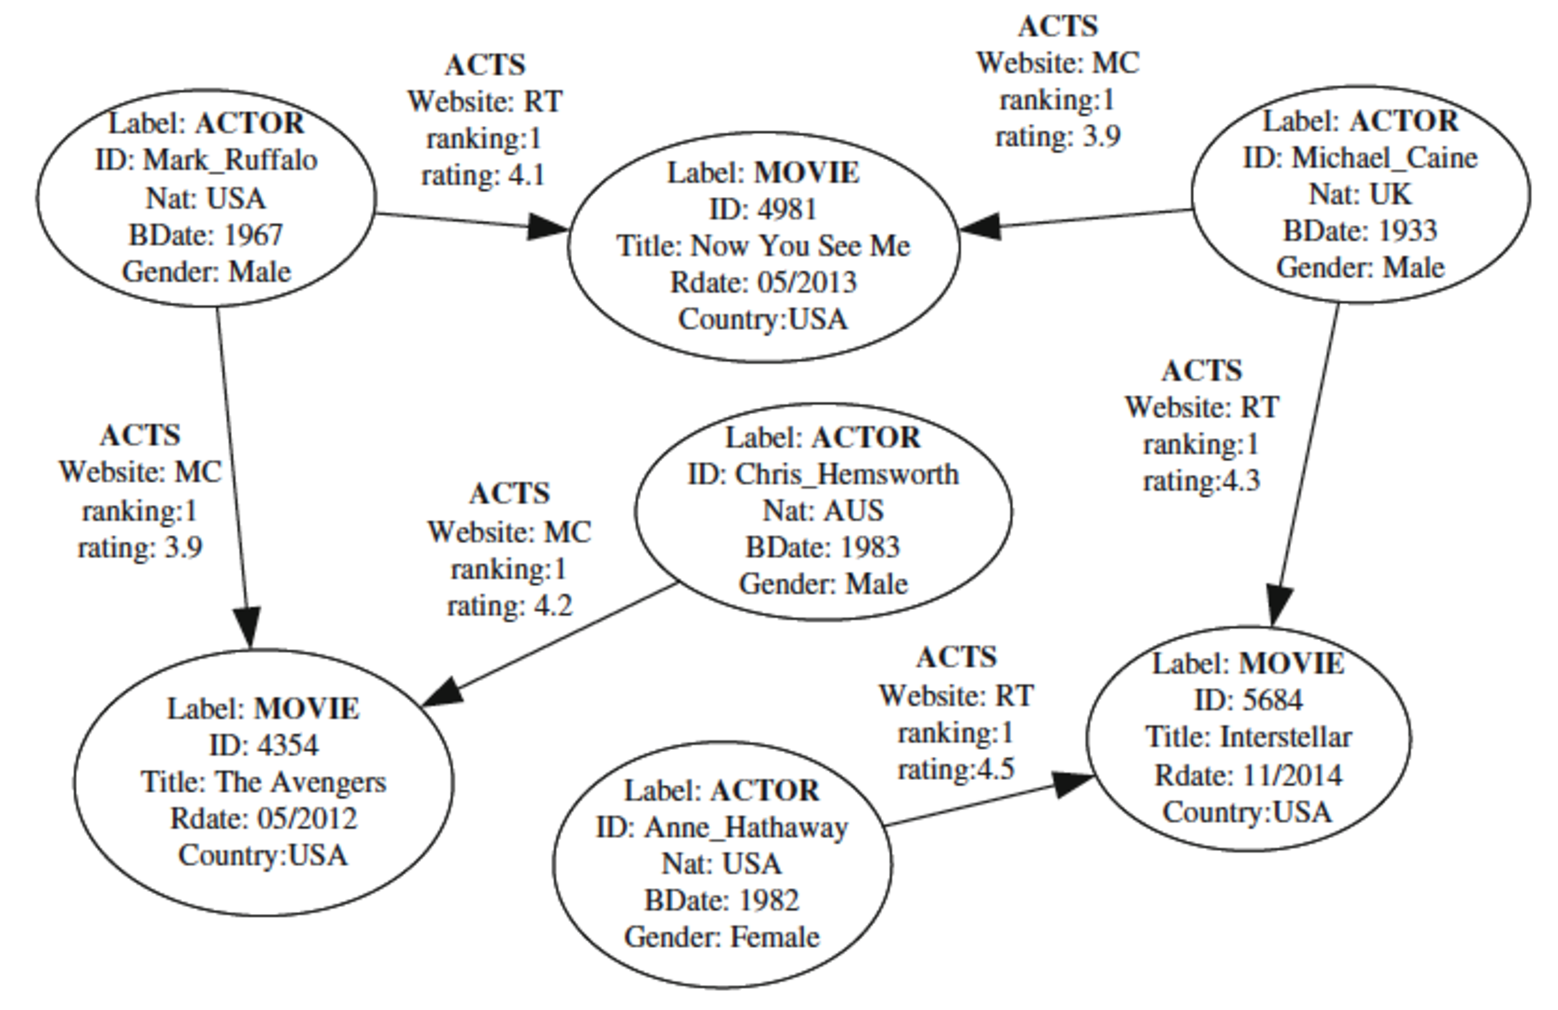
\includegraphics[width=0.8\textwidth]{../movie_graph.png}
\caption{Original movie graph \cite{ghrab2015framework}}
\label{fig:figure21}
\end{figure}

Once the dimensions are selected, a graph lattice is defined by all possible OLAP aggregations obtained by aggregating the intra-class dimensions. The inter-class measures fall back in one of the aforementioned categories (content-based,  graph-specific or graph as measure).

Figure \ref{fig:figure22} shows the aggregate graph obtained by grouping movies by their release date and actors by their birth date and gender. The graph shows the average ranking and rating of the ACTS relationship between grouped actors and movies.

\begin{figure}[ht]
\centering
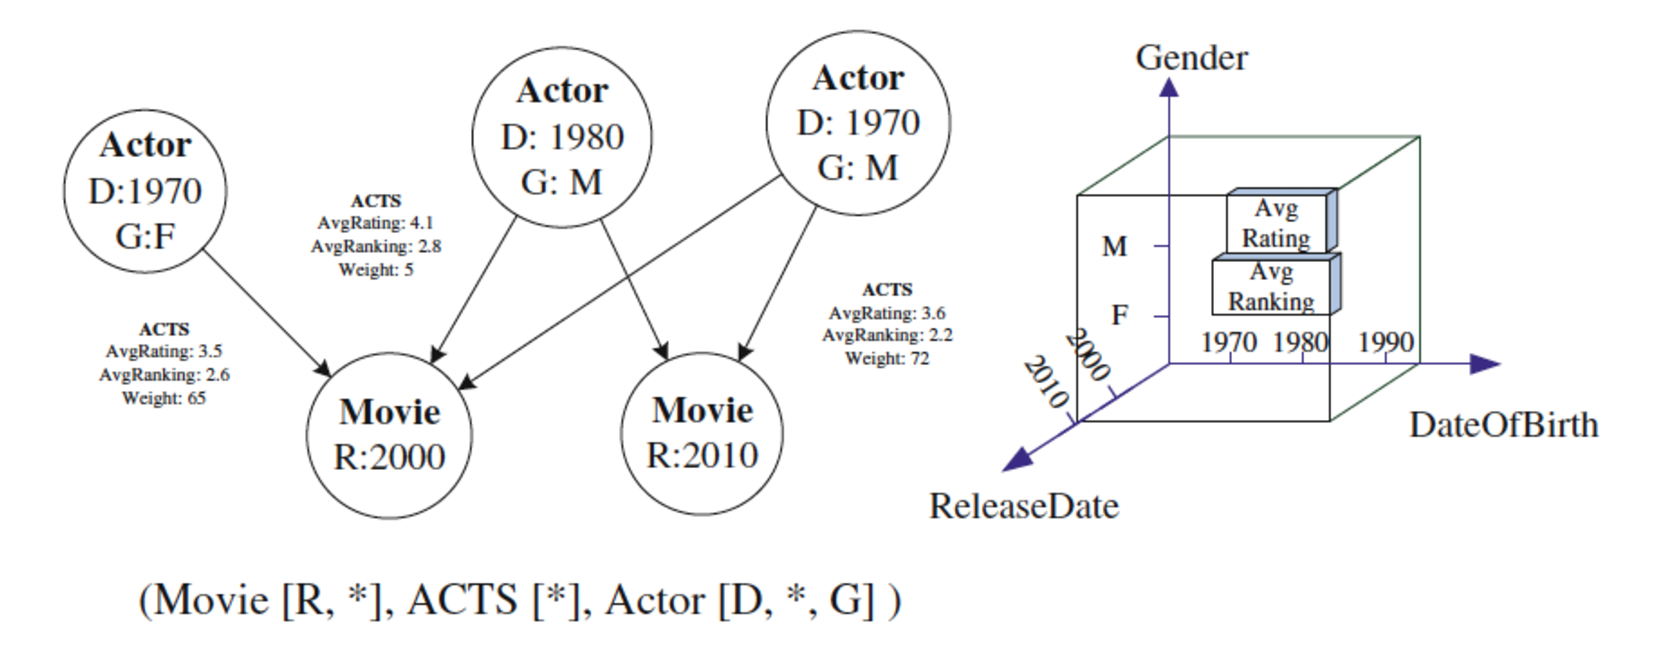
\includegraphics[width=1\textwidth]{../interclass_dimension.png}
\caption{Aggregate Graph for inter-class dimensions \cite{ghrab2015framework}}
\label{fig:figure22}
\end{figure}

This paper also proposes a technique for building OLAP cubes extracted from a graph modelled according to the analysis-oriented graph database model GRAD. This model provides advanced graph structures, integrity constraints and graph algebra. According to the authors, traditional property graphs only support OLAP analysis of inter-class dimensions, while additional capabilities brought by GRAD allows the analysis of information stored within each vertex.
 
The GRAD model consider heterogeneous, attributed, labelled graphs and supports complex type attributes on the vertices. This model introduces special analytical structures called hypernodes, that represent real world entities grouped by classes. Each hypernode is a subgraph formed by an entity vertex - which contains the label and the identifier attributes - attributes vertices - linked to the entity vertex and represent the non-identifier attribute - and literal vertices - which stores the effective value of its attribute vertex. Figure \ref{fig:figure23} shows an example of a movie graph modelled with GRAD.

\begin{figure}[!h]
\centering
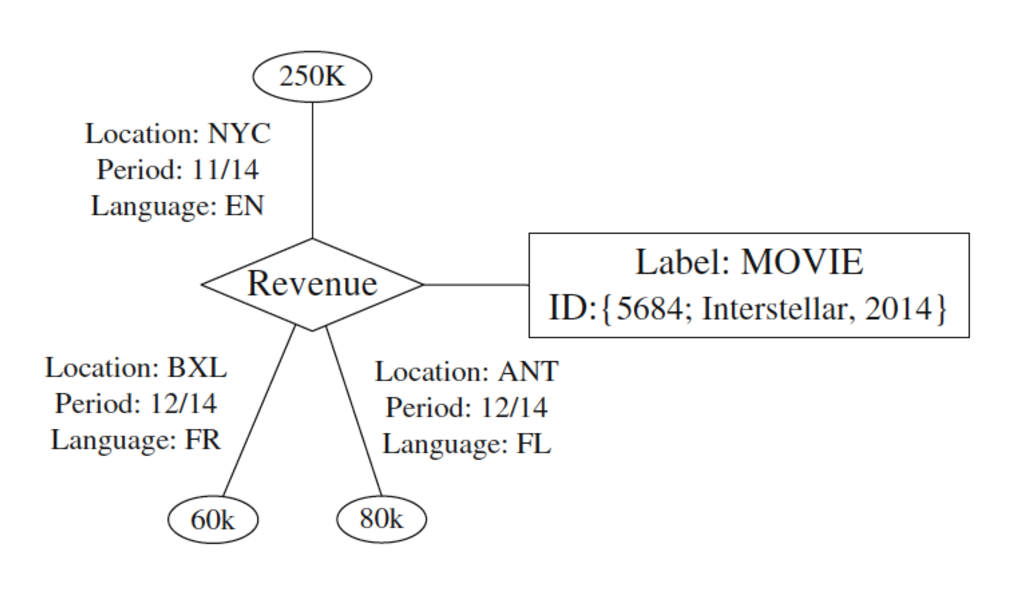
\includegraphics[width=0.5\textwidth]{../grad_model.png}
\caption{Movie graph on GRAD model \cite{ghrab2015framework}}
\label{fig:figure23}
\end{figure}

Based on this model, the paper defines Intra-class Dimensions as a subset of attributes vertices. The Intra-class Measures are identified by the attribute vertex label and are calculated in a similar way as the measures in property graph model. Figure \ref{fig:figure24} shows the result of applying aggregation function to the original GRAD graph in order to calculate the revenue measure, aggregating the Location according to the Country Name (CN) attribute.

\begin{figure}[!h]
\centering
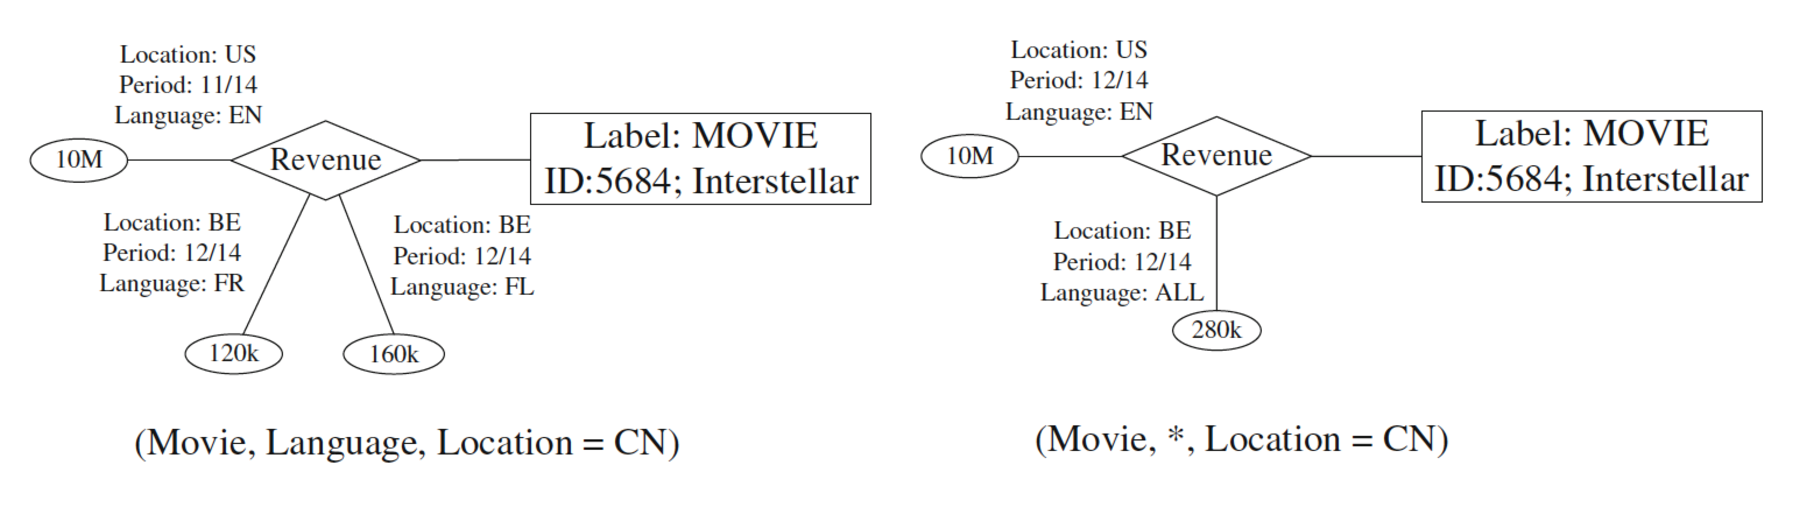
\includegraphics[width=1\textwidth]{../intraclass_dimension.png}
\caption{Aggregate Graph for intra-class dimensionl \cite{ghrab2015framework}}
\label{fig:figure24}
\end{figure}

This framework's implementation used Neo4J for the graph storage and HDFS  (Hadoop Distributed File System) for distributed processing. The architecture is also composed by a middleware layer that is responsible for computing the aggregate graph and measures, using GraphX\footnote{https://spark.apache.org/graphx/} library to calculate graph-specific measures.

\section{Comparative Analysis}

The first works done in OLAP analysis on graph focused on homogeneous graph datasets and defined ground concept of this area, such as aggregate graphs and graph lattice. Several operators were proposed and, in general, three types of measures were taken into consideration:
\begin{description}
\item[Informational / Content-based / Attribute-based measure] Similar to traditional OLAP measures, this information is obtained by applying an aggregate function on the vertex's attributes.
\item[Topological / Aggregate Graph measure]  This type of measure gives information about the topology of the graph and is obtained by applying aggregate function on vertices and edges, generating a graph as a measure.
\item[Graph-based / specific measure] This type of measure is based on graph analysis theory and can be represented by a number or a subgraph.
\end{description}

One relevant characteristic of the works presented so far is the little explanation given on how the framework was indeed implemented, which made their understanding rather difficult. The Table \ref{tb:table1} shows a comparison between all the frameworks presented in this chapter, regarding the type of graph, dimensions and operations supported by each one.

\begin{table}[!ht]
\setlength\extrarowheight{2pt}
\caption{Comparison of studied frameworks}
\label{tb:table1}
\begin{tabularx}{\textwidth}{|Y|Z|Z|Z|}
\hline
\cellcolor[HTML]{C0C0C0}\textbf{Framework} & \cellcolor[HTML]{C0C0C0}\textbf{Graph} & \cellcolor[HTML]{C0C0C0}\textbf{Dimensions} & \cellcolor[HTML]{C0C0C0}\textbf{Operations}\\\hline
{\cellcolor[HTML]{EFEFEF} Graph Cube} & Homogeneous & Vertex Attributes & Cuboid and Crossboid Query\\\hline
{\cellcolor[HTML]{EFEFEF} Graph OLAP} & Homogeneous & Informational and Topological & I-OLAP and T-OLAP Operations\\\hline
{\cellcolor[HTML]{EFEFEF} HMGraph} & Heterogeneous & Informational, Topological and Entity & I-OLAP, T-OLAP, Rotate and Stretch Operations\\\hline
{\cellcolor[HTML]{EFEFEF} Pagrol} & Homogeneous & Vertex and Edge Attributes & 3 Query Category and Roll-up/Drill-down Operations \\ \hline
{\cellcolor[HTML]{EFEFEF} GRAD Graph Cubes} & Heterogeneous & Inter-class and Intra-class & - \\ \hline
\end{tabularx}
\end{table}

The work proposed here will be focused in heterogeneous graph datasets and will support the three types of measures described previously, in a similar way as presented by the work on GRAD Graph Cubes. In addition to that, this work will also explore OLAP operations and network analysis on graph databases without the need to define a new graph model, as suggested by previous works, eliminating the extra step of parsing operational data to the new model.

\section{Final Considerations}

In this chapter, we presented the main research works published related to OLAP system using Graph Databases. The majority of the works available only supported homogeneous graph, but they introduced important concepts of the area, such as graph cubes and aggregate graph. The implementations that actually gave support to heterogeneous graph, proposed different graph models in order to answer analytical queries. In the next chapter, we will specify a simple OLAP system using Graph Database without the need to define a new graph model.
